\subsection{Trituración $S_4$}

El sistema de trituración es un sistema manual del compostador, de ahí el nombre sistema semi-automatico.

La potencia con la que trabaja este sistema de trituración esta directamente relacionado con la fuerza que un ser humano puede generar al girar un brazo de palanca, por lo que el sistema esta limitado en gran medida en comparación de lo que sería un sistema totalmente automático accionado por un motor (\ref{fg:brazo}).


\begin{figure}[h!]
            \centering
            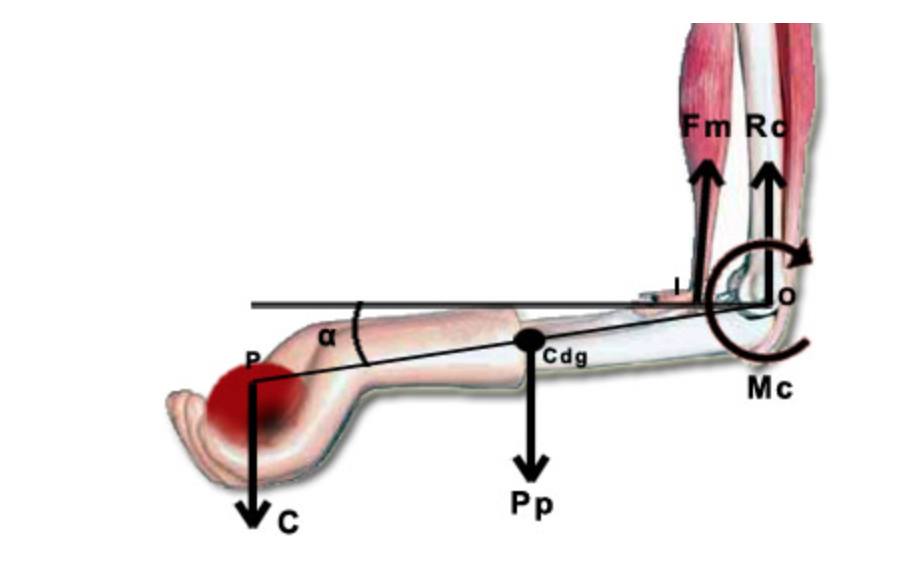
\includegraphics[scale=0.5]{images/Capitulo 4/S4/Brazo de Palanca Humana.png}
            \caption{Brazo de Palanca Humana}
            \cite{Biomec}
            \label{fg:brazo}
\end{figure}

\subsubsection{Momento generado por un humano}

La fuerza nominal $F_n$ que puede generar el brazo de un humano es de \cite{Biomec}:

\begin{center}
    $F_n = 8.5 \frac{kg}{cm^2}$
\end{center}

Considerando la longitud estándar de un brazo humano, se puede generar un momento $M_c$ de \cite{Biomec}:

\begin{center}
    $M_c = 66.7 Nm$
\end{center}

Al considerar la anchura del compostador, se tiene que el brazo de palanca $L$ más grande posible es:

\begin{center}
    $L = 0.3 m$
\end{center}

Por lo que la fuerza máxima queda definida por:

\begin{center}
    $F_{max} = \frac{M_c}{F_n}=\frac{66.7}{0.3} = 222.33 N$ \\
    $F_{max} \approx 222.5 N $
\end{center}

Esta fuerza es suficiente sabiendo que no se trituraran huesos, y la materia orgánica más dura a moler serán cascaras de sandía.

Sabiendo todo esto, se procedió a buscar una solución en el mercado que se adaptara a las necesidades del proyecto. 

Después de una amplia búsqueda, se determinó que un molino manual de carne se adaptaba de manera correcta al proyecto.

El molino seleccionado cumple con la capacidad de trituración que se busca tener, este triturador, (figura \ref{fg:molino}), es capaz de procesar hasta 82 kilogramos de carne por hora.

\begin{figure}[h!]
            \centering
            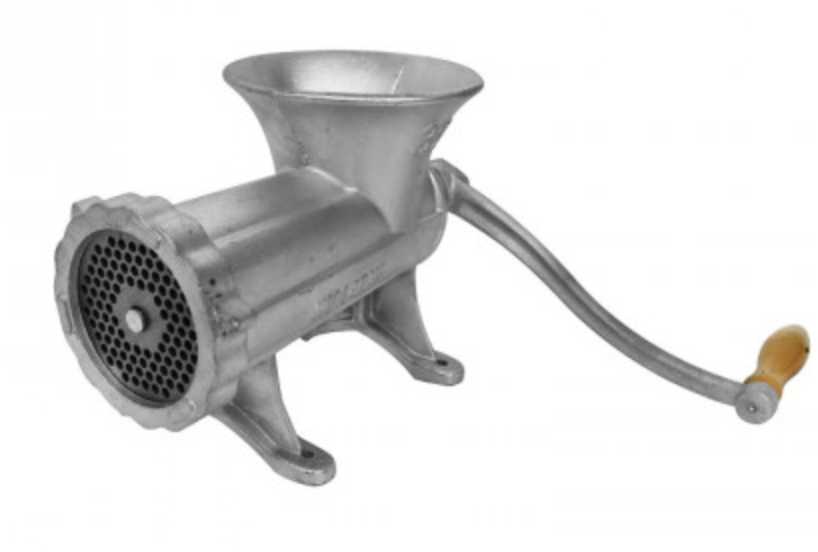
\includegraphics[scale=0.8]{images/Capitulo 4/S4/Molino 32.png}
            \caption{Molino de carne manual}
            \label{fg:molino}
\end{figure}



\subsubsection{Validación del sistema de trituración}

Para validar el componente seleccionado, se verificó el tamaño de las partículas a la entrada y a la salida, teniendo a la entrada del sistema una abertura ovalada de un diámetro mínimo de 5 centímetros, por lo que a la entrada del sistema se puede insertar la materia orgánica a procesar sin ningún tipo de problema.

A la salida se encuentra un disco ranurado , cual puede ser cambiado de acuerdo a nuestras necesidades, el molino de carne ya viene con un disco ranurado con orificios de 5mm de diámetro, lo cual permite obtener a materia orgánica lista para su procesamiento con una dimensión menor a la máxima permitida. 

\begin{figure}[h]
            \centering
            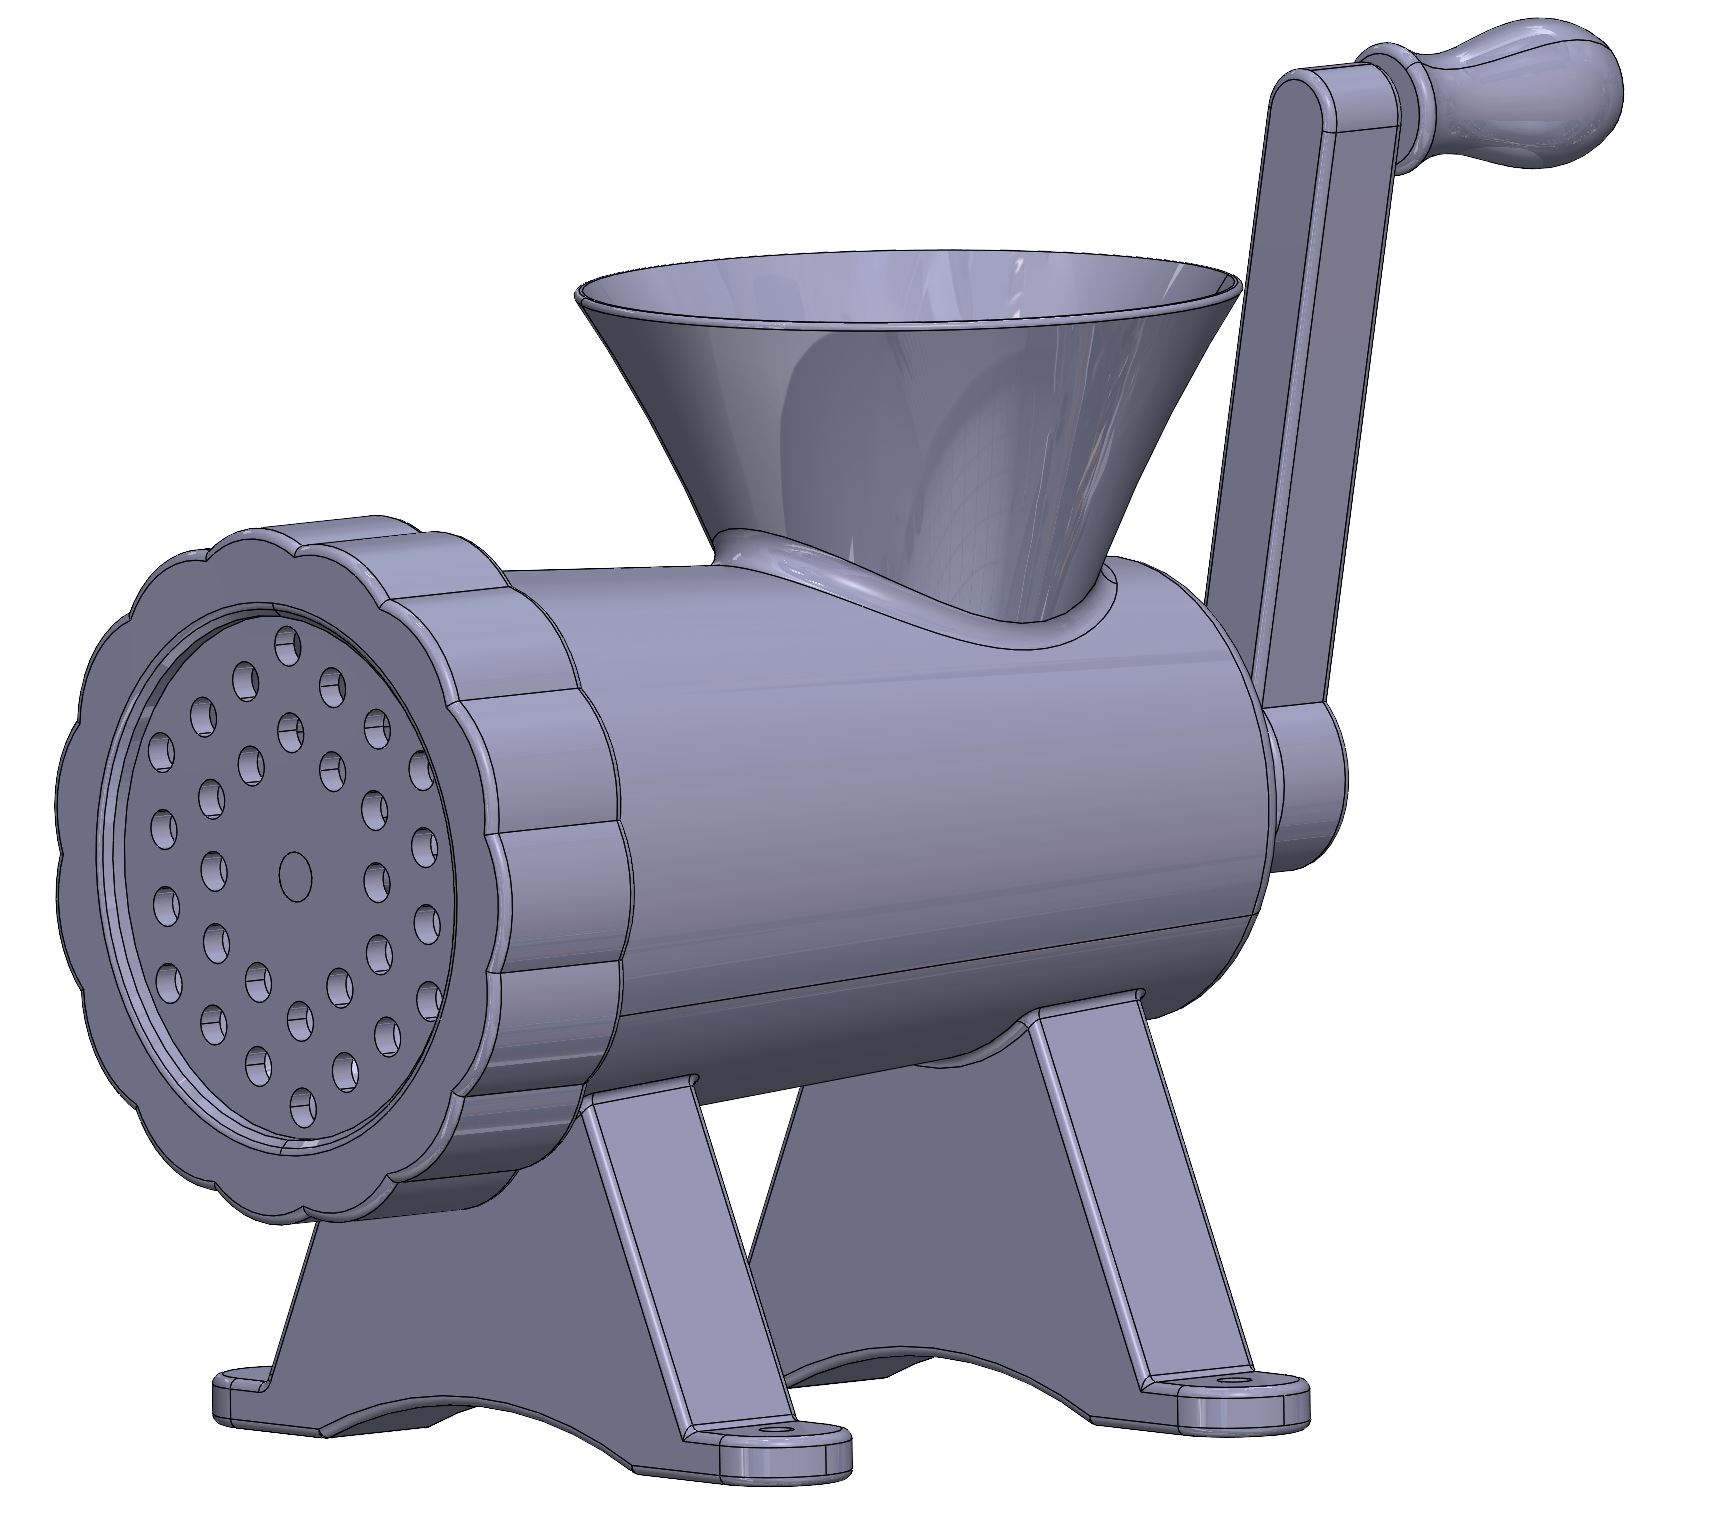
\includegraphics[scale=0.3]{images/Capitulo 4/S4/Modelo-CAD-triturador.png}
            \caption{Modelo CAD del molino de carne manual}
            \label{fg:molinoCAD}
\end{figure}

El molino consiste en un disco helicoidal de paso variable encargado de ir presionando la materia orgánica hacia el disco ranurado, en el eje va montada una cuchilla que ayuda a cortar la materia orgánica en trozos pequeños que puedan fácilmente salir por las ranuras del disco.